This chapter provides important artifacts related to design of our project.

\section{Software Design}

This section presents the UML class diagram and gives a brief description of each class in our system. Attributes and methods of each class and relationship among classes are clearly presented.

Figure \ref{fig:UML_Unity} describes the UML of the software made in Unity 3D. The \texttt{SoftwareController} acts as the main controller of the entire engine and is also responsible for \texttt{GET} and \texttt{POST} requests to the firebase database, whereas the \texttt{VideoController} and \texttt{SliderController} are used for viewing video and gives its control options. The rest of the controllers are Screen Controllers which are child objects to \texttt{Screen} type gameobjects made in Unity. These controller of each screen is defined according to the activity involved in that interface. 

Figure \ref{fig:UML_PoseEvaluation} describes the UML of the pose evaluation module. \texttt{Features} class is responsible for extracting the features out of \texttt{PoseData} objects constructed through \texttt{.csv} files generated by \texttt{PoseEstimator} class. The \texttt{Features} class uses \texttt{SmoothingFilter} for data smoothing and filtering and for getting derivatives. These extracted features are used by \texttt{PoseEvaluator} class which temporaly aligns the necessary features and generates feedback. The feedback is generated on the basis of individual feature scores provided by \texttt{PoseEvaluator}. 

\begin{figure}
  \centering
  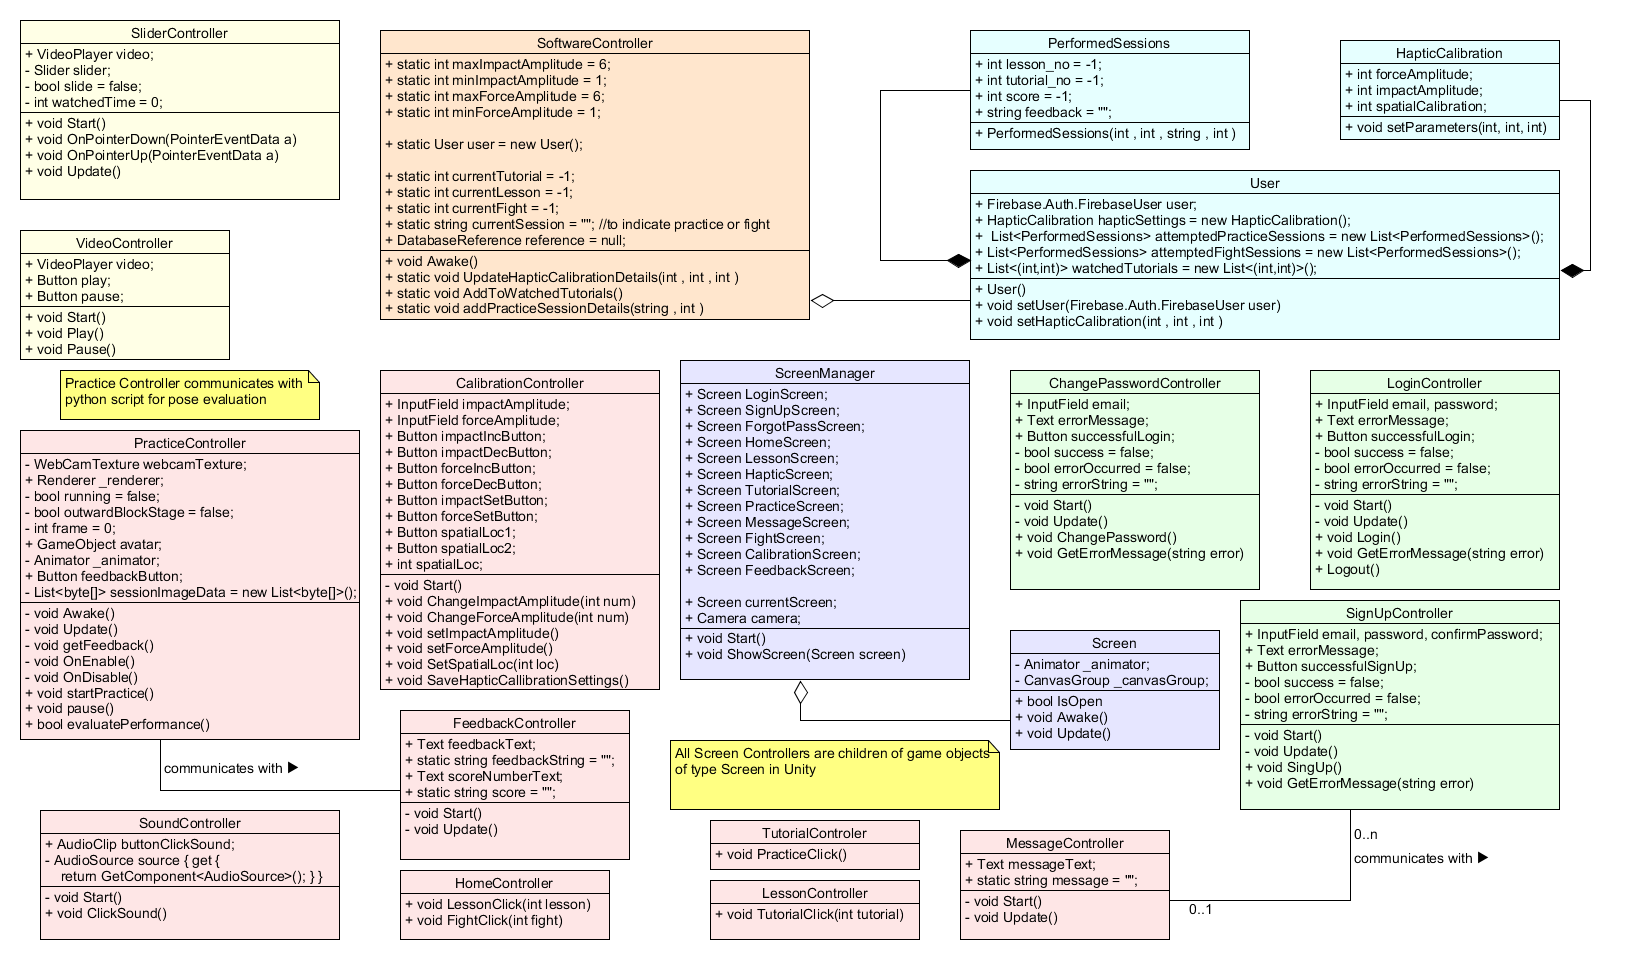
\includegraphics[scale=0.3]{images/UML - Unity Software.png}
  \caption{UML of the Unity Software}
  \label{fig:UML_Unity}
\end{figure}

\begin{figure}
  \centering
  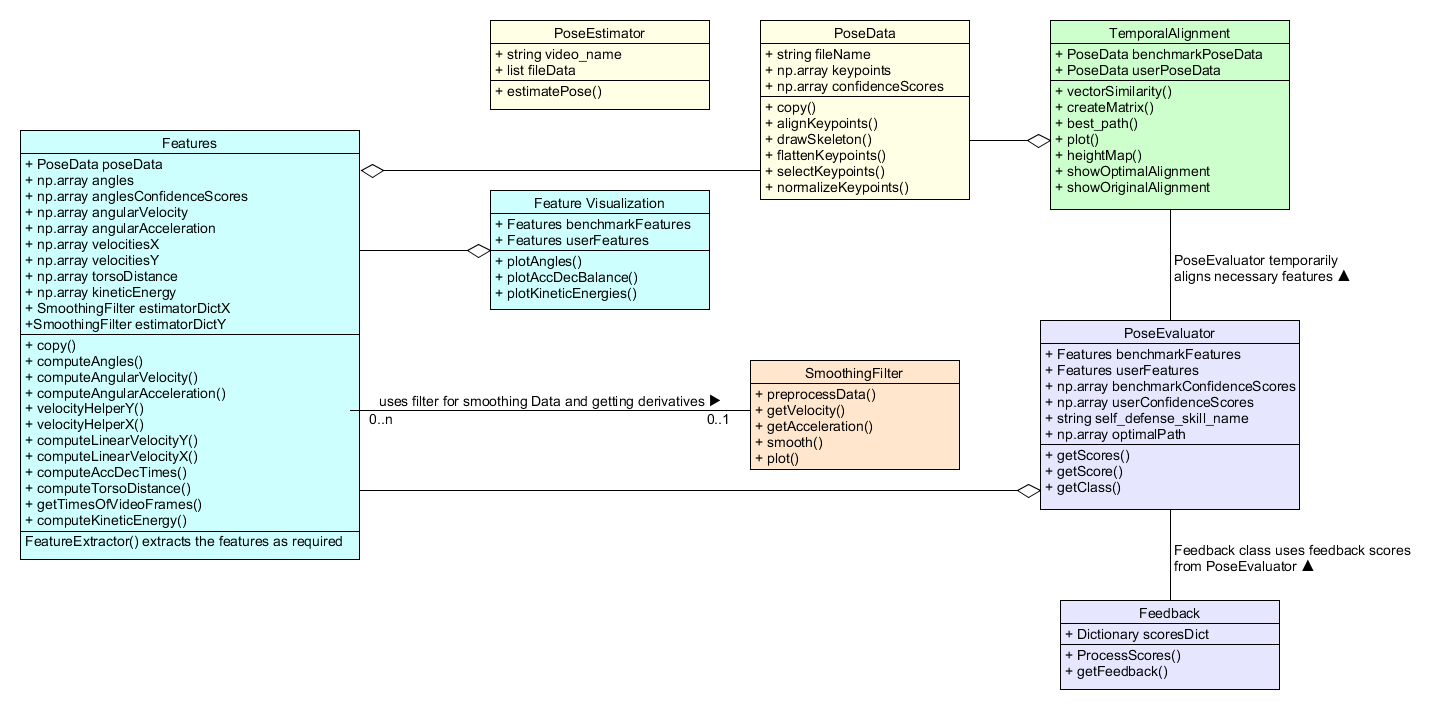
\includegraphics[scale=0.34]{images/UML - Pose Evaluation Module.png}
  \caption{UML of the Pose Evaluation Module}
  \label{fig:UML_PoseEvaluation}
\end{figure}


% Your report will contain ONE of the following 2 sections.

\section{Data Design}

This section presents the structure of our database that caters to persistent data storage in our project. The structure is shown in figure \ref{fig:RelationalDatabase} is a normalized data model for relational databases. It clearly shows entities, attributes, relationships with their cardinalities, and primary and foreign keys. We have used DB designer to build our data model.


Each user will have a username and password. We need to save the so far progress of the user, for example, how many tutorials they have watched, how many practice and fight sessions they attempted and what score and feedback they received in those and what settings of haptics they calibrated according to their comfort level. In addition to user based data, we also need to store which video and animated tutorial to display in which tutorial and practice session, because these tutorial and practice screens have the same GUI, only their animation changes. If a user has attempted a fight session, we also need to store what tutorials were suggested to them by the system, in case the user feels the need to go back to them. For pose classification and evaluation, we also need to store benchmark videos of different self-defense moves along with their extracted key-points. Their extracted features are stored in a different table because many different features can be extracted from each move. 

\begin{figure}
    \centering
    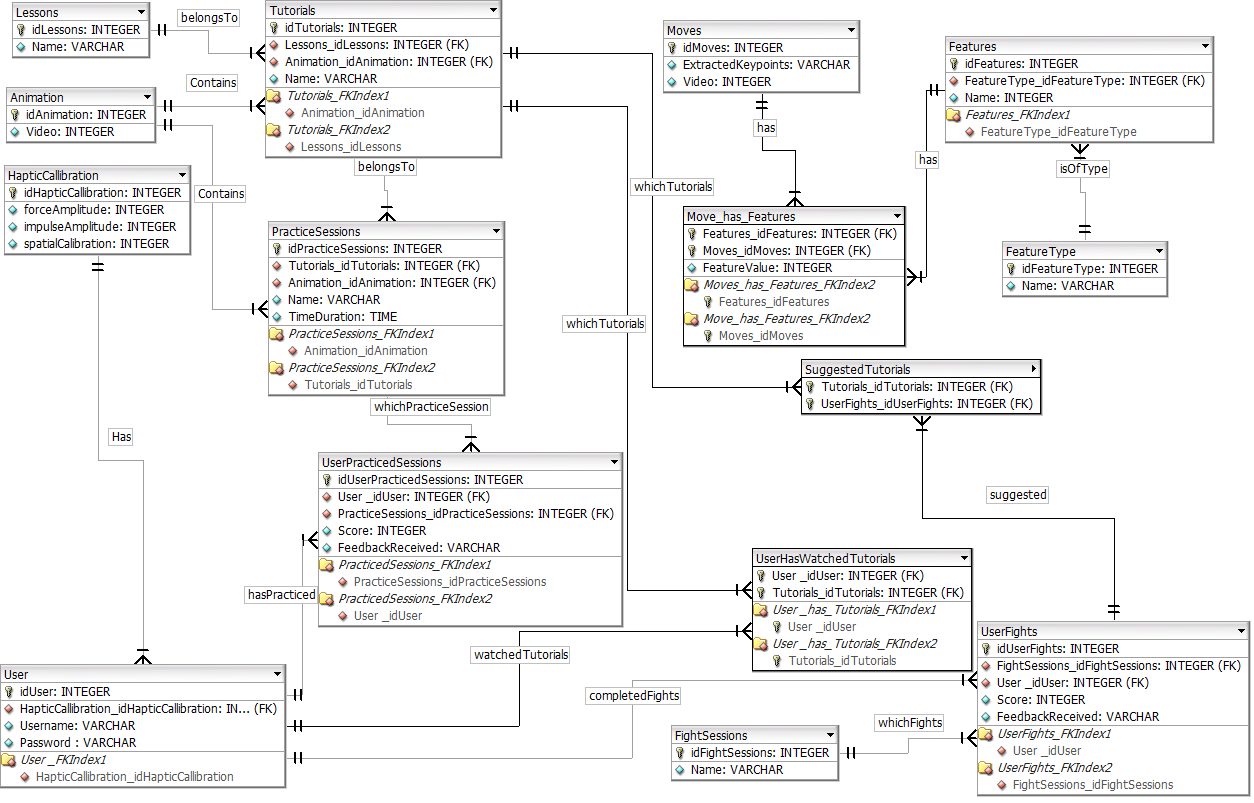
\includegraphics[scale=0.38]{images/databaseDesign.png}
    \caption{Relational Database}
    \label{fig:RelationalDatabase}
\end{figure}


\section{User Interface Design}
The user interface is built on unity game engine. 
Figure \ref{fig:credentials} shows the user interface for handling user authentication and updating credentials. The authentication is done via using Firebase Authentication SDK for Unity by manually integrating their authentication methods into the unity software. It is an email and password based authentication which authenticate users with their email addresses and passwords. The Firebase Authentication SDK provides methods to create and manage users that use their email addresses and passwords to sign in, and it also handles sending password reset emails. 

\begin{figure}
    \centering
    \subfigure[Login Screen]{% 
      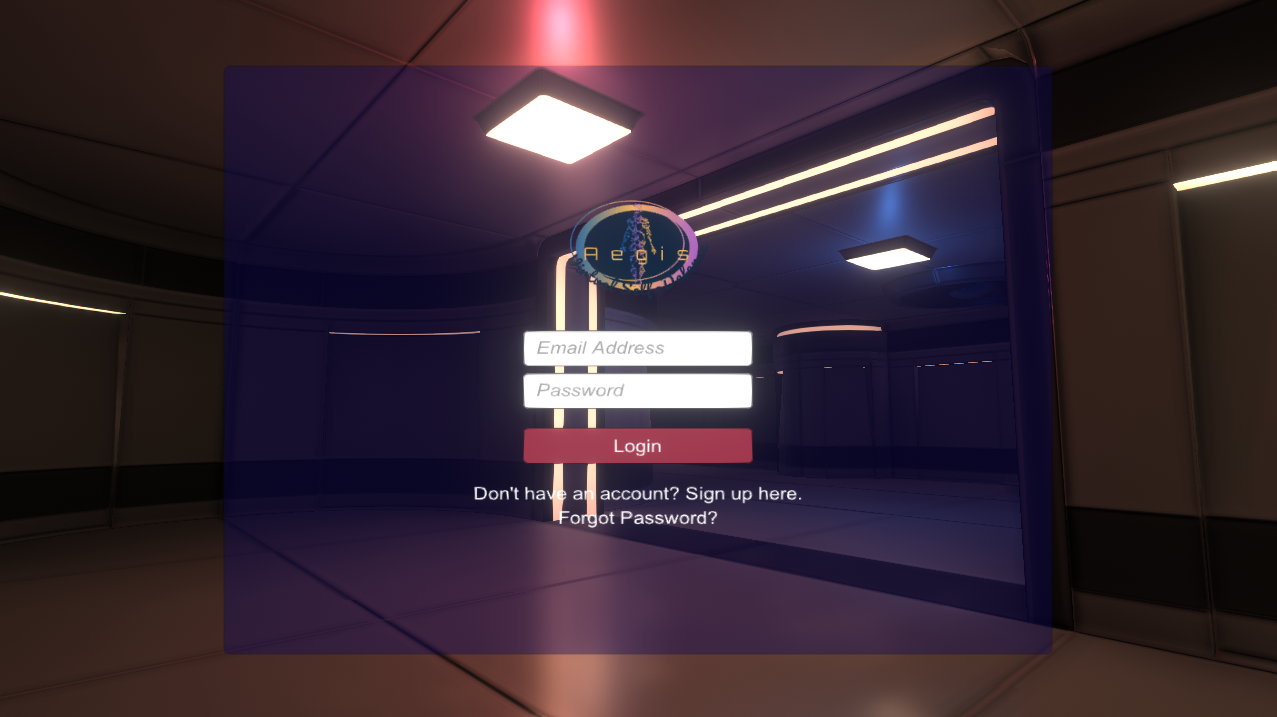
\includegraphics[scale=0.31]{images/screens/login.png} \label{fig:loginUnity} 
    } 
   \quad 
    \subfigure[SignUp Screen]{% 
     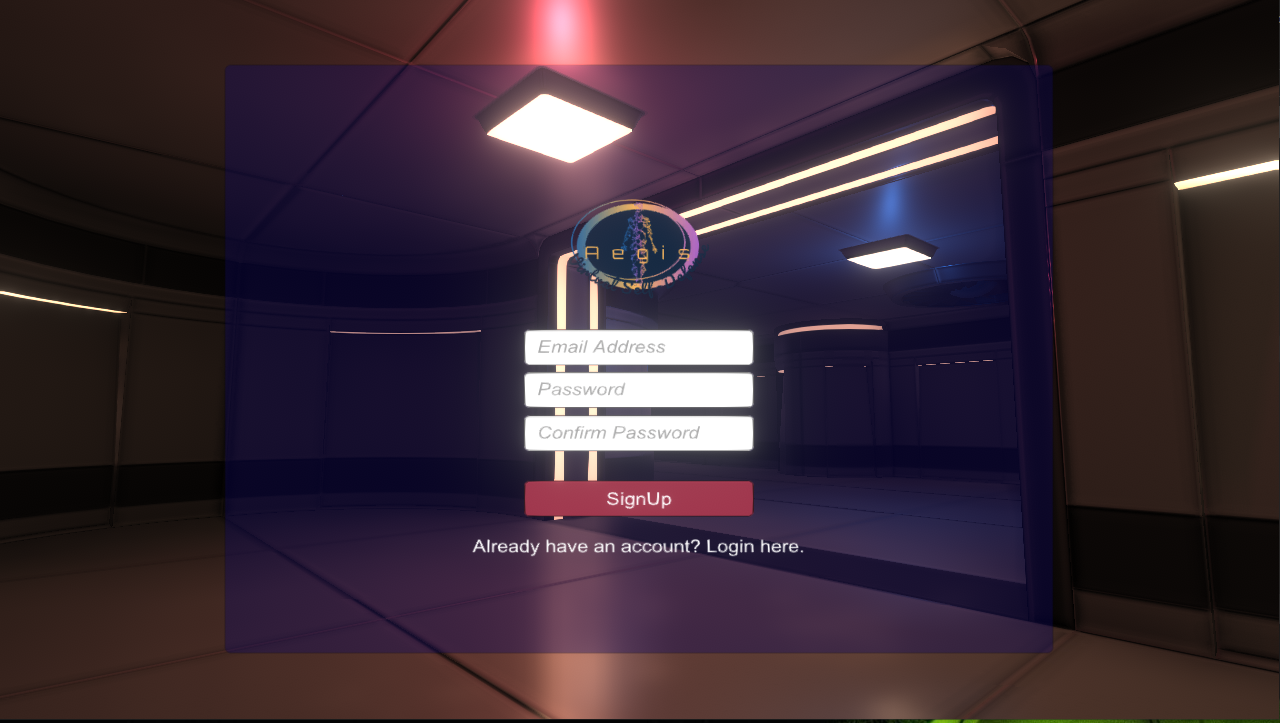
\includegraphics[scale=0.31]{images/screens/signUp.png}     \label{fig:signUp} 
    } \\
    \quad 
    \subfigure[Forgot Password Screen]{% 
      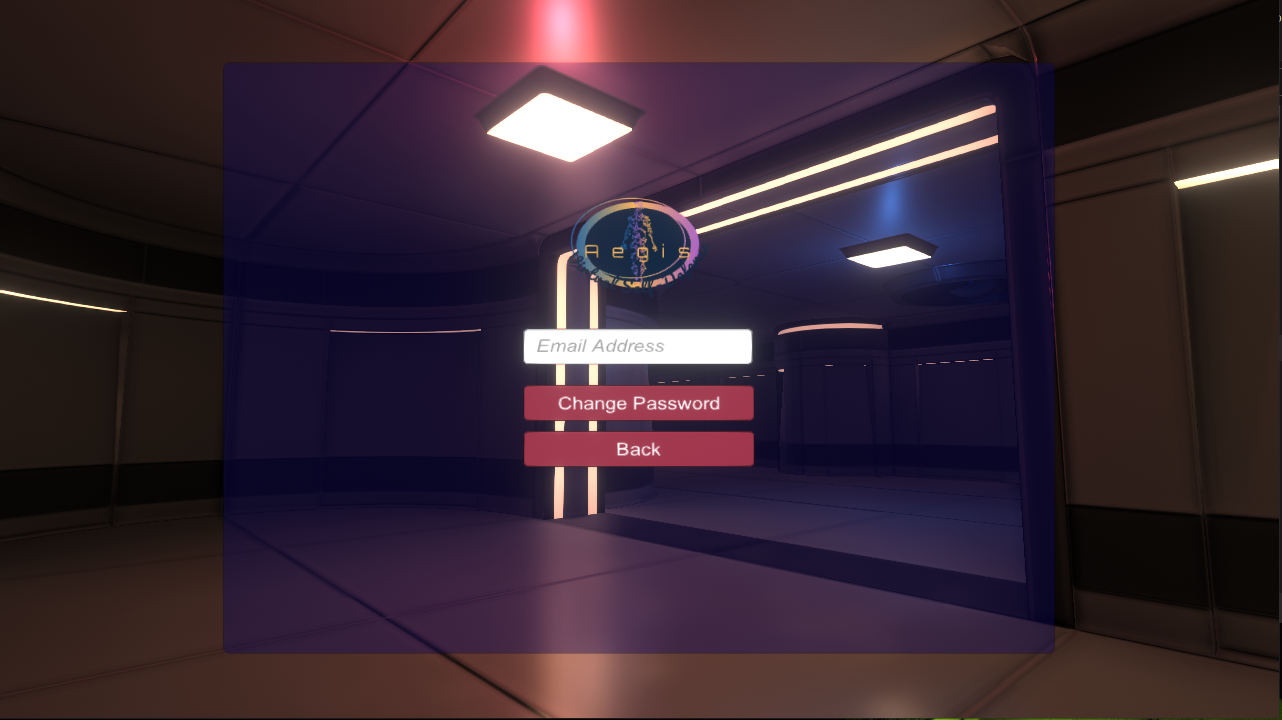
\includegraphics[scale=0.31]{images/screens/forgotPassword.png} 
      \label{fig:forgotPassword} 
    }
    \caption{User Interface for Authentication} 
    \label{fig:credentials}
\end{figure}

Figure \ref{fig:homeScreen} shows the main menu (home screen) display when the user is granted access to the system. The home screen gives the user the option to either select training mode or fighting mode. 

\begin{figure}
    \centering
    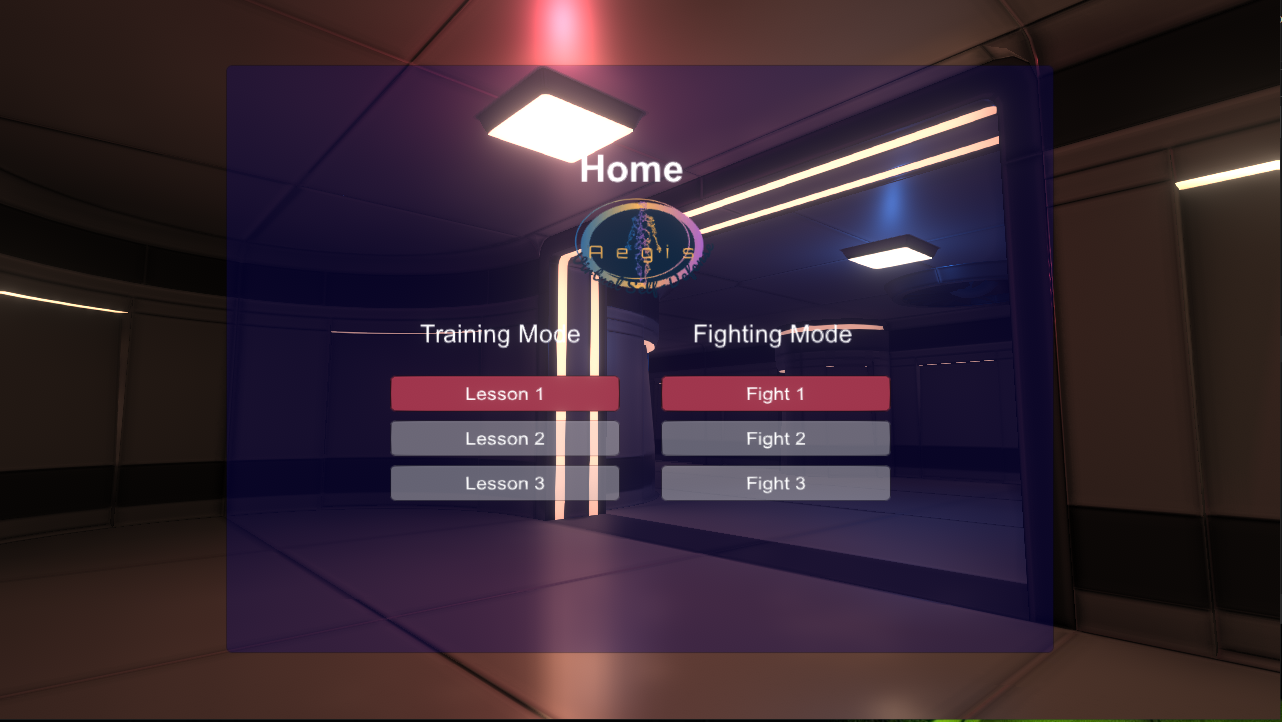
\includegraphics[scale=.5]{images/screens/home.png}
    \caption{User Interface for Main Menu}
    \label{fig:homeScreen}
\end{figure}

Since our system is modular, it allows the liberty of practising without the haptic suit. However, without it, the software won't be able to give full human trainer like realistic experience. This option solely exists to cater to those not comfortable in wearing the haptic suit. Therefore, before proceeding to any practice or fight session, the system prompts the user to select their preference as shown in figure \ref{fig:hapticPrompt}. In case the user chooses to practice with the haptic suit, the software requires haptic calibration prior to proceeding any further as shown in figure \ref{fig:hapticCallibration}. The user must calibrate amplitude as well as the spatial position of electrodes as anatomical variations are the biggest limitation of EMS. Once calibrated, these settings will be stored in the Firebase Database. 

\begin{figure}
    \centering
    \subfigure[Haptic Prompt Screen]{% 
      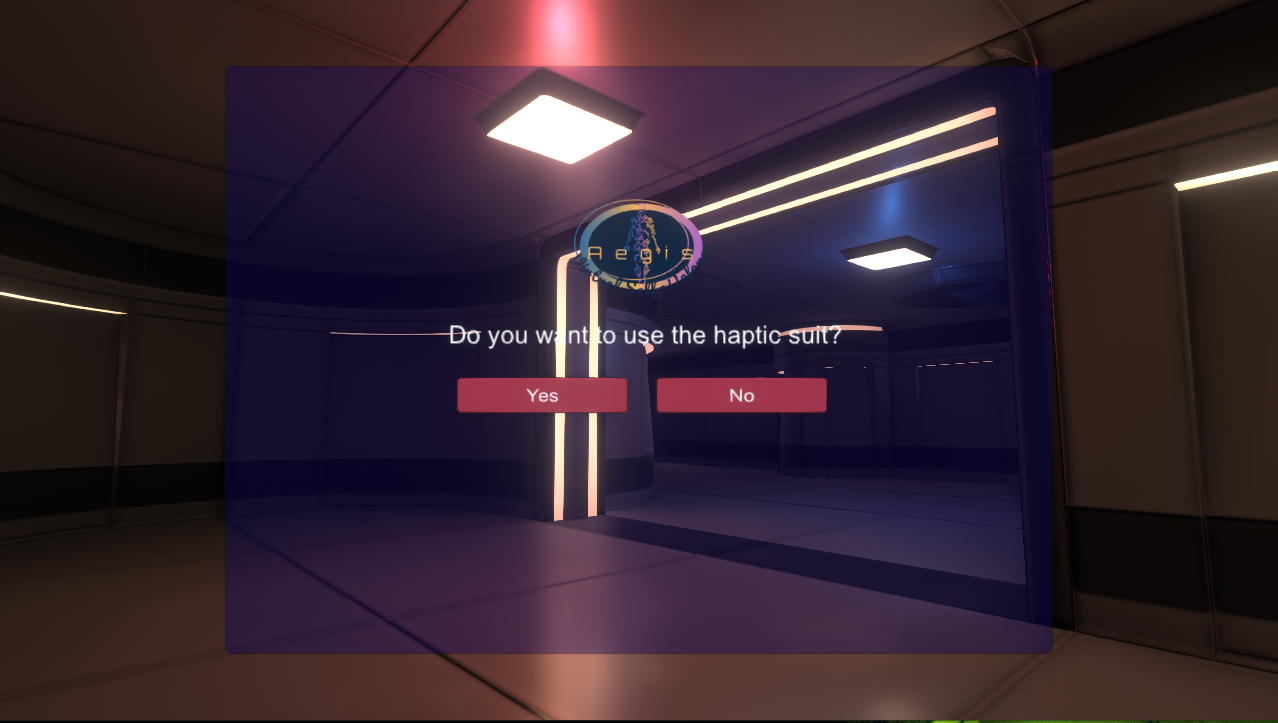
\includegraphics[scale=0.31]{images/screens/hapticPrompt.png} 
      \label{fig:hapticPrompt} 
    } 
   \quad 
    \subfigure[Haptic Callibration Screen]{% 
     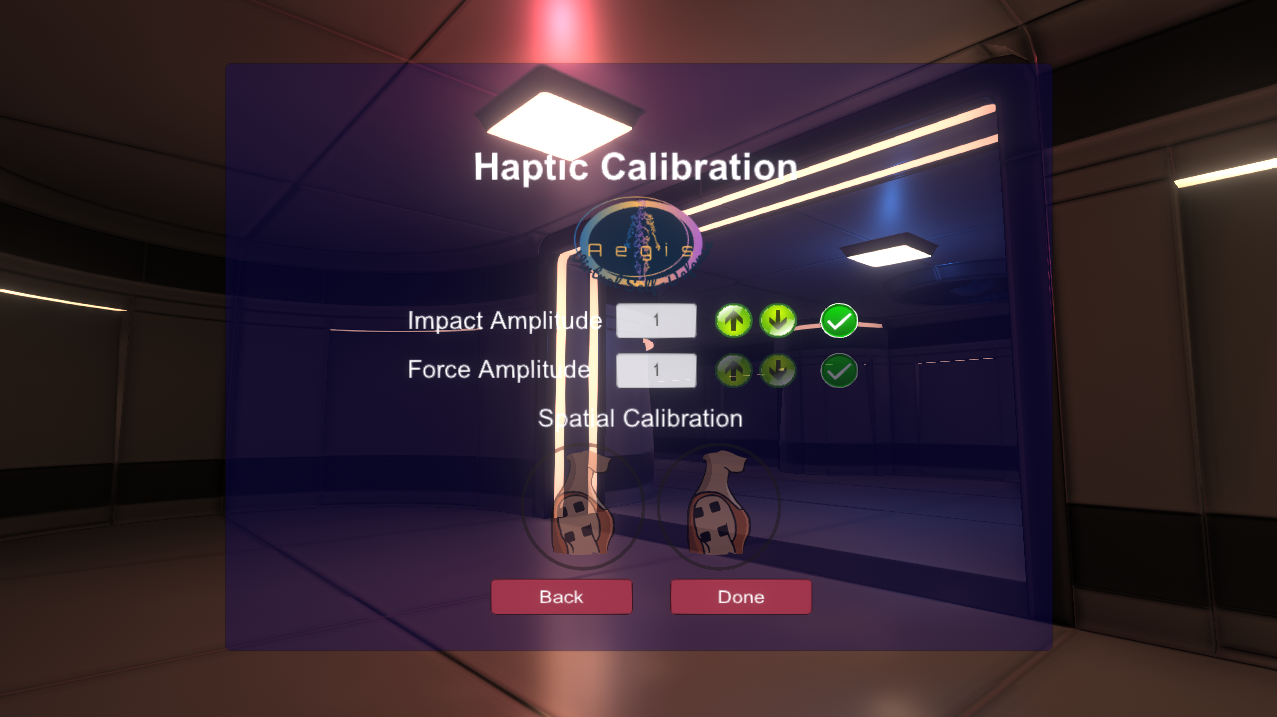
\includegraphics[scale=0.31]{images/screens/hapticCallibration.png}     
     \label{fig:hapticCallibration} 
    }
    \caption{User Interface for Selecting and Calibrating Haptics} 
    \label{fig:hapticScreen}
\end{figure}

Figure \ref{fig:tutorials} shows the user interface for lessons and tutorials. The training mode contains lessons, tutorials and practice sessions, whereas the fighting mode contain fight sessions of corresponding lessons. Each tutorial teaches a specific skill through a video as shown in figure \ref{fig:tutorialUnity}. 

\begin{figure}
    \centering
    \subfigure[Lessons Screen]{% 
      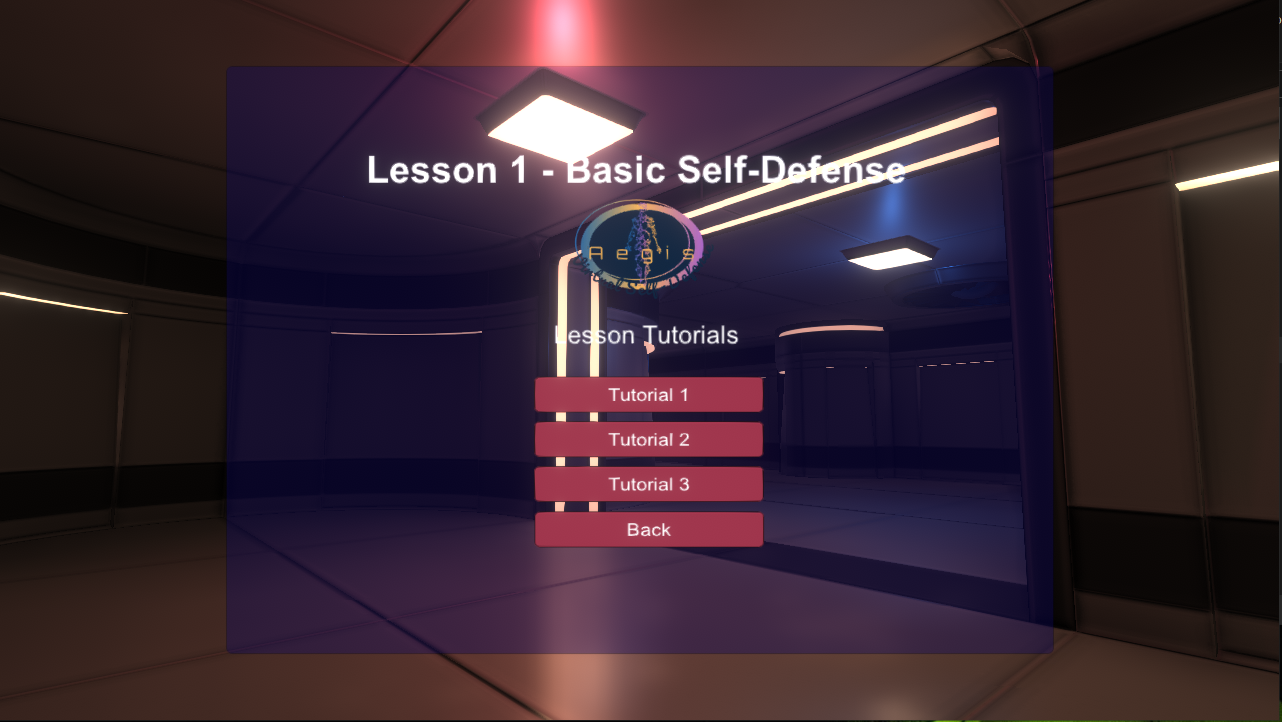
\includegraphics[scale=0.3]{images/screens/lesson.png} \label{fig:lessonUnity} 
    } 
    \quad 
    \subfigure[Tutorial Screen]{% 
      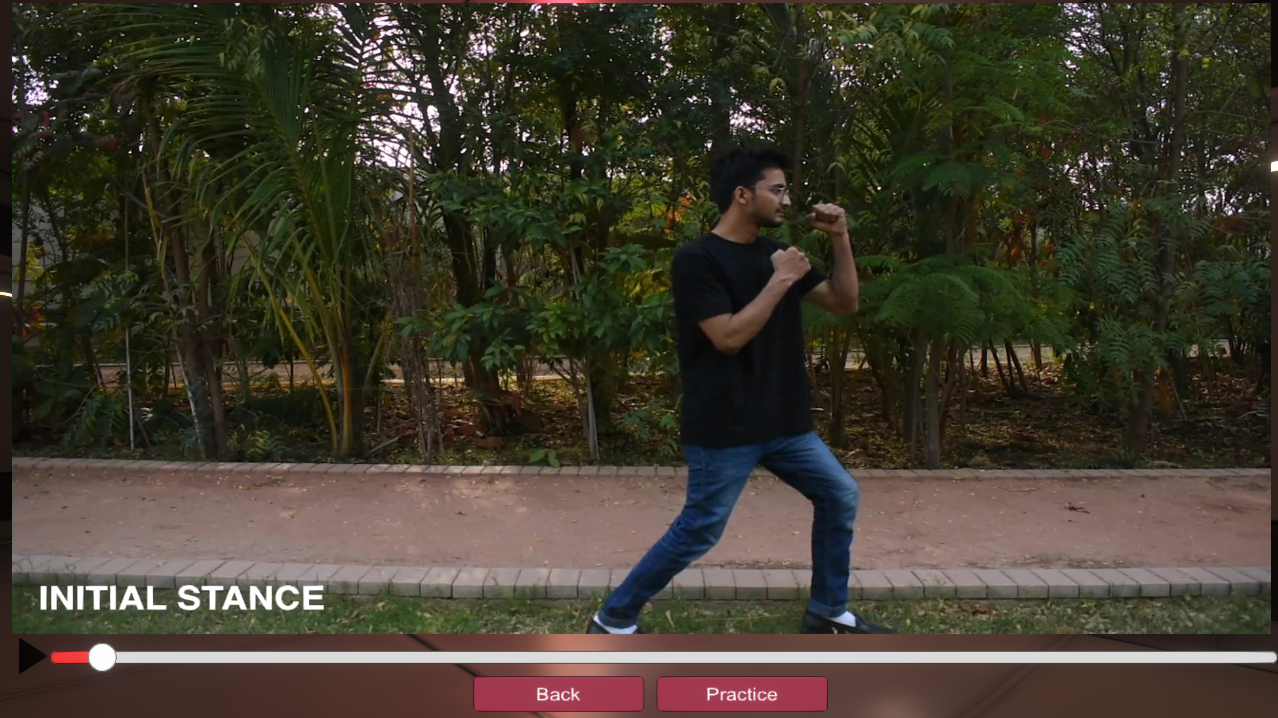
\includegraphics[scale=0.3]{images/screens/tutorial.png} \label{fig:tutorialUnity} 
    }
    \caption{User Interface for Lessons and Tutorials} 
    \label{fig:tutorials}
\end{figure}

For practice and fight sessions, an animated avatar attacks the user, requiring them to attack the avatar back in defense based on the skills taught. These practice and fight sessions are started when a button click event is triggered by the user, which then signals the hardware and starts extracting image frames of the user through webcam, see figure \ref{fig:practiceAndFightSessions}.

\begin{figure}
  \centering
  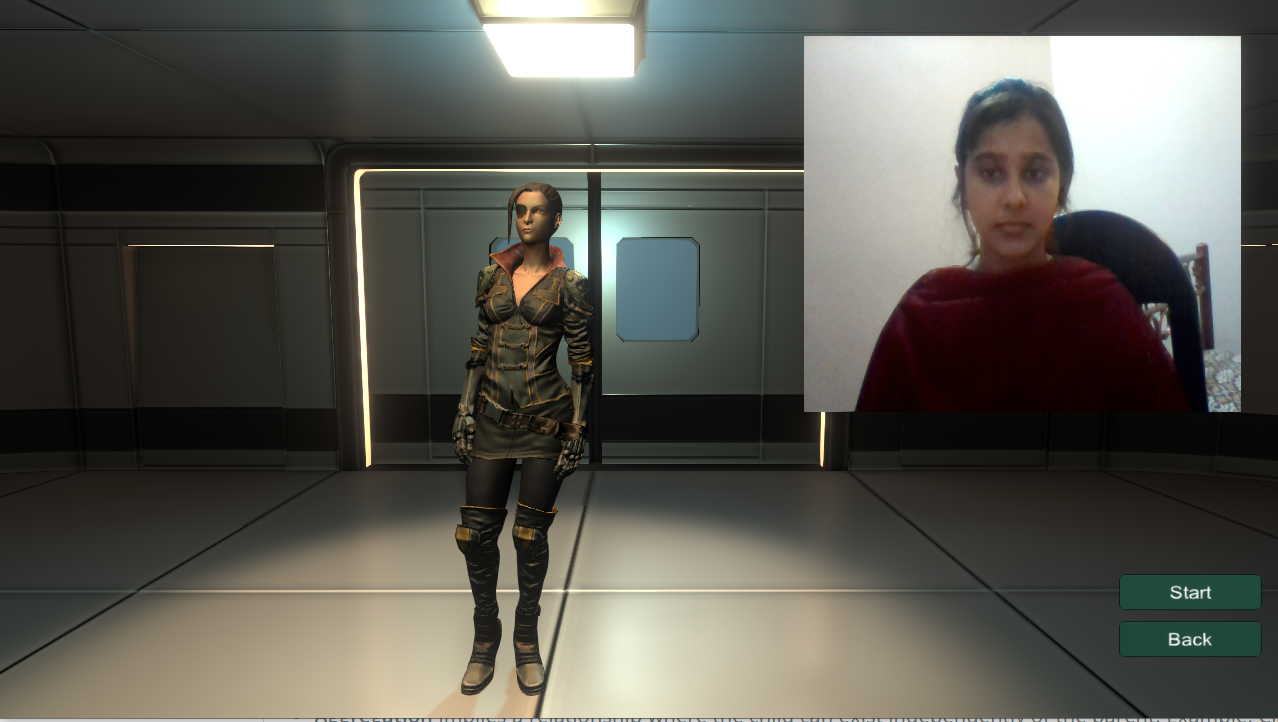
\includegraphics[scale=0.5]{images/screens/practice.png} 
  \caption{User Interface Practice and Fight Sessions} 
  \label{fig:practiceAndFightSessions}
\end{figure}

When the avatar animation has ended, unity communicates with the python script which then evaluates the user pose and gives feedback to the user. Figure \ref{fig:feedbackScreen} shows the feedback provided to the user after a practice session.

\begin{figure}
  \centering
  \subfigure[Feedback Provided to the User]{% 
    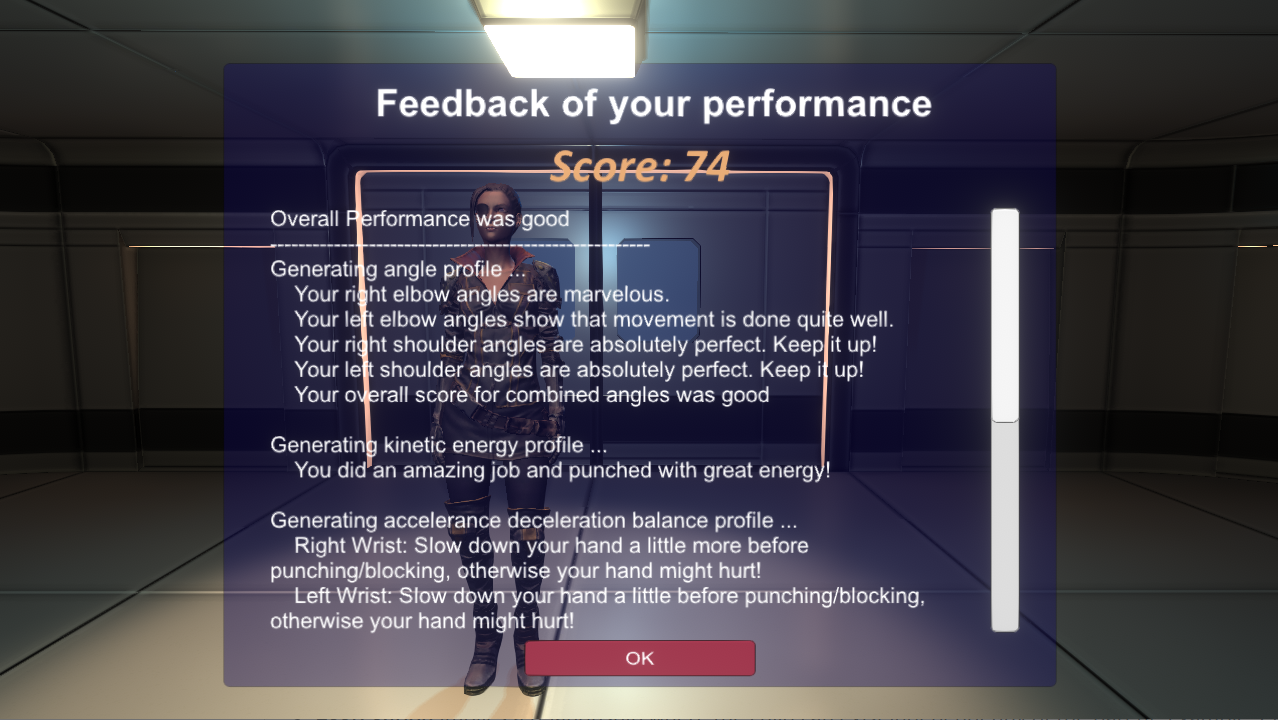
\includegraphics[scale=0.3]{images/screens/feedback1.png} \label{fig:feedback1} 
  } 
 \quad 
  \subfigure[Feedback Continued]{% 
   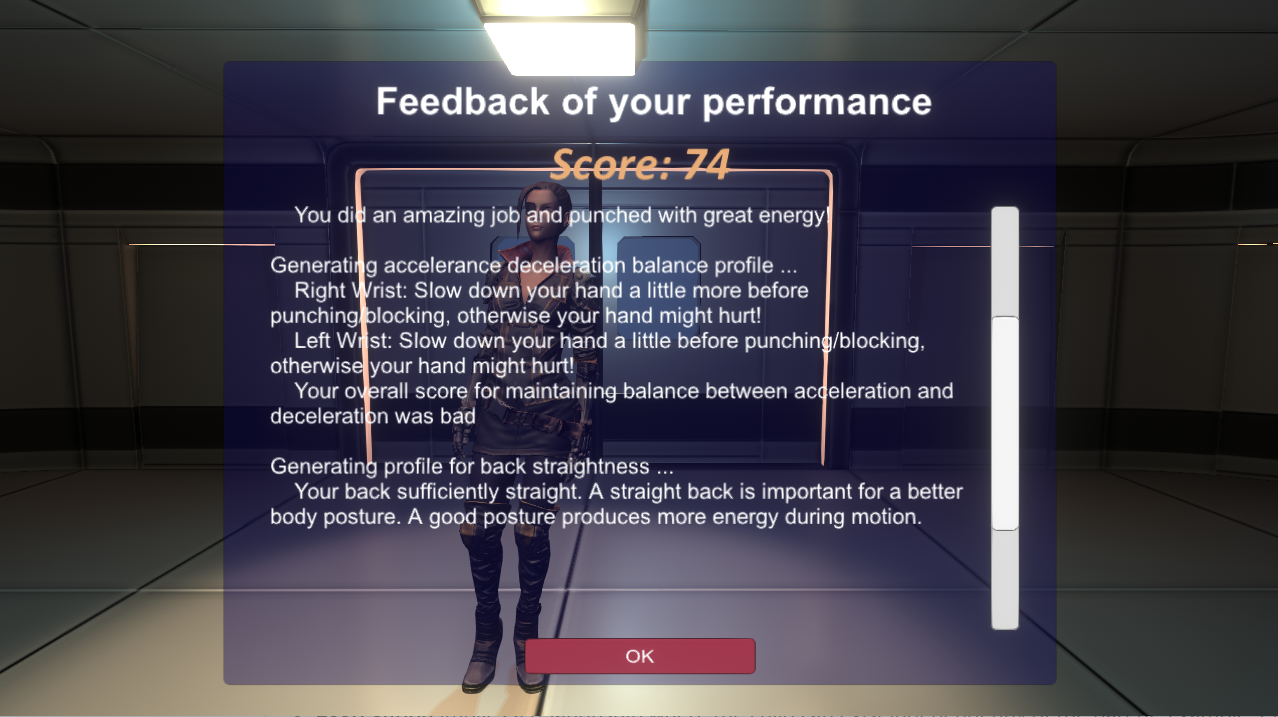
\includegraphics[scale=0.3]{images/screens/feedback2.png} 
   \label{fig:feedback2} 
  } 
  \caption{User Interface for Feedback Screen} 
  \label{fig:feedbackScreen}
\end{figure}


\section{Haptic Feedback Hardware Design}

The haptic feedback comprises of Electric muscle stimulation (EMS) source, the Transcutaneous electrical nerve stimulation (TENS) machine, and electrodes placed on the body. The hardware pipeline begins with an RGB camera capturing human images, during practice and fight sessions, at 30 fps and openpose producing the pose vector. To check if a user hits avatar, the wrist coordinate in the pose vector is checked if it collides with the avatar's bounding box. In case of a collision, a trigger is sent to an arduino system. This is the base of the hardware. This system activates the already calibrated TENS machine signals, at user specified spatial set of electrodes and amplitude level. In case of collision, it gives an impulse on the fist giving a sense of tap. It also locks the elbow by contracting the biceps/triceps. This contracting of muscles causes the arm to fold across the elbow joint. This gives an impression of arm being locked, since it is coupled with a person forcing a punch into the virtual avatar. Figure \ref{fig:punchSimulation} shows the placement of electrodes on arms and fists responsible for giving impulse on fists as an indication that some collision has occurred, and for locking the arm to prevent penetrating into the virtual objects. 

\begin{figure}
    \centering
    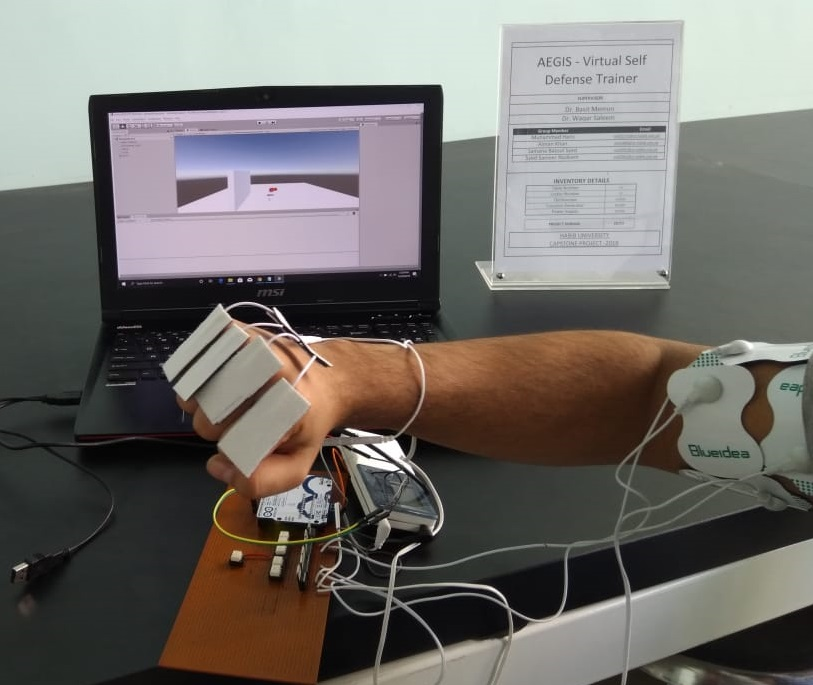
\includegraphics[scale=.7]{images/setup.jpg}
    \caption{Simulating a punch in the virtual world.}
    \label{fig:punchSimulation}
\end{figure}

The TENS machine we are using is the 'Digital TENS BE-660', a low frequency Digital TENS developed by Besmed. This device is connected with an Arduino Uno which communicates with unity through serial communication. The communication is one-way, that is, only Unity sends data to the arduino. The figure \ref{fig:besmed} shows the TENS machine and its components used.

\begin{figure}
    \centering
    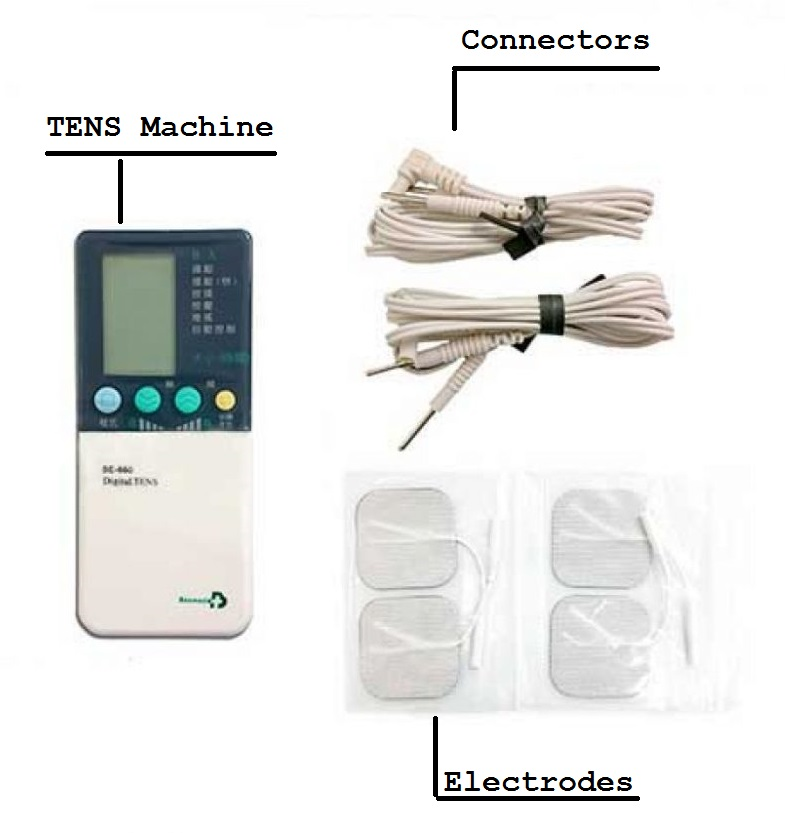
\includegraphics[scale=.5]{images/Besmed1.jpg}
    \caption{TENS Machine basic}
    \label{fig:besmed}
\end{figure}

The anatomical variations are the biggest limitation of designing a versatile haptic system using EMS. However, we have tried to overcome that hurdle by offering different spatial modes for electrodes and intensity levels. Due to the current pandemic we were not able to test our system robustly for a large number of people. We did however test it on a smaller set of people, which gave an affirmative response to the haptic feedback. 

\section{Scoring Mechanism Pipeline}

As mentioned in the earlier sections system captures user's pose via a single RGB web camera and then computes a stick figure on each frame, via openpose, an returns a $18 \times 3$ matrix for each frame. Figure \ref{fig:stickFigure} shows stick figure of the human being superimposed on the original frame. These keypoints are compared with the keypoints obtained from the bench mark video sequence in order to compare the user movements. The scores assigned to user are relative to the benchmark performance. The procedure of assigning scores is not real time, the pose evaluation process runs after the user's performance has ended hence we do not need to output results in less than a second. 

\begin{figure}
    \centering
    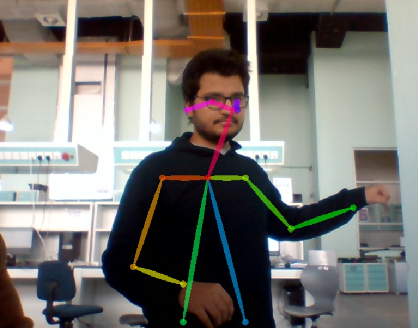
\includegraphics[scale=.75]{images/sketeton.png}
    \caption{Stick figure from openpose superimposed on original frame}
    \label{fig:stickFigure}
\end{figure}

Following are the different parts involved in pose evaluation.

\subsection{Pose Estimation}
When a practice or fight session ends, unity communicates with the python script responsible for estimating poses through openpose, on the images extracted through webcam during the session; %see Appendix \ref{appendix:code}. 
The pose estimation data is stored in a \texttt{.csv} file format that is used scoring mechanism for pose evaluation. 

\subsubsection{Openpose Parameters}
We have used "COCO" pose model that is trained on COCO dataset, and a net resolution of $-1 \times 80$ as the GPU machine did not allow for a net resolution greater than this due to insuffient memory, as described in section \ref{sub:designConstraints}. The number of maximum people that can be detected while pose estimation has been limited to just one, as we only need to detect one user only. The keypoint scaling has been set to 3 that normalizes all the estimated keypoints on a unit square from 0 to 1. 

\subsubsection{Writing Pose Data}

For each frame, 18 keypoints are extracted, and each keypoint is a 2D joint location along with the confidence score of that keypoint, hence each keypoint can be represented as \texttt{(x,y,CS)} where \texttt{CS} is the confidence score. The confidence scores are in the range [0,1]. Therefore, each frame data is represented as a $18 \times 3$ matrix. If openpose does not detect any human in a frame, then a $18 \times 3$ null matrix is pushed to the file. For $n$ frames, the \texttt{.csv} file contains $n \times 18$ rows of data. 

\subsubsection{Coordinate Transformation}
Openpose's coordinate system is different from python's coordinate system, hence all the keypoints are transformed to align with python's coordinate system so visualizing the data is clearer. 

\subsection{Feature Extraction}

After pose estimation, the next task in the pipeline is to extract revelant features from  the data. Since we have only incorporated punch-block sequence in the project yet, the features are defined only for punch-block sequence. These features might change based on any other self-defense technique. For the punch-block sequence \cite{karatePunch} we have extracted the following features:

\begin{enumerate}
  \item Right shoulder and elbow angles 
  \item Left shoulder and elbow angles 
  \item Torso distance for calculating straightness of the back
  \item Kinetic energy 
  \item Acceleration and deceleration balance for biomechanical efficiency. 
\end{enumerate}

\subsubsection{Shoulder Angles}
Shoulder angles are calculated to make sure the user has performed the shoulder movements correctly. Correct shoulder movements are necessary for a proper punch. For example, if a user punches without displacing the elbow to the back first, then the punch looses most of its power and force. This displacing of elbow towards the back is captured by shoulder angle opening wide, and then shrinking again as the hand moves forward until it crosses the limbs, after which it starts to increase again. 

Shoulder angles are calculated through the equation \ref{eq:angle} where the middle joint becomes the origin, and $k_n, k_s$ and $k_e$ represents the neck, shoulder and elbow keypoints, and $J_{n,s}$ and $J_{e,s}$ represents the segments from neck  and elbow to shoulder respectively. 

\begin{gather}
  \textit{Neck to Shoulder Joint Segment}: J_{n,s} = K_n - K_s \\
  \textit{Shoulder Origin}: J_{s,s} = K_s - K_s = O \\
  \textit{Elbow to Shoulder Joint Segment}: J_{e,s} = K_e - K_s \\
  \alpha = cos^{-1} \big (\dfrac{J_{n,s} \cdot J_{e,s}}{||J_{n,s}|| ||J_{e,s}||})
  \label{eq:angle}
\end{gather}

These angles are computed for every frame, however the keypoint values are first filtered before extracting angles; section \ref{section:filteringSmoothing} talks more about filtering data. 

To calculate the score based on angles, we can not simply compare them with benchmark angles, as the probability that two users will produce perfectly aligned movements even if they are performing the exact same action, is extremely low. To solve this misalignment issue, dynamic time warping is used to temporally align the data of user and benchmark, this is described in detail in section \ref{section:dtw}

After dynamically warping the timed sequences of angles, the difference scores between both angle arrays are computed by calculating the absolute difference between them as shown in equation \ref{eq:angleDiffScore}. 
%However, the angle arrays are first multiplied by their confidence scores for each frame as shown in equation \ref{eq:angleTimesCS} where $A$ is the angle array and $CS$ is its confidence scores array, and the multiplication happens element-wise. The confidence score of an angle for frame $m$ contained by keypoints $K_{i,m}, K_{j,m}, K_{k,m}$ are calculated through equation \ref{eq:angleCS} where $CS_{i,m}, CS_{j,m}$ and $CS_{k,m}$ are confidence scores of keypoints $i,k$ and $k$ for frame $m$. 
These difference scores are then normalized to get on scale of 0-1 by dividing by the max difference score as shown in equation \ref{eq:normalizedAngleDiff}, and the similarity score is computed by subtracting 1 from it. 

%\begin{align}
  %\alpha_m = CS_{i,m} \cdot CS_{j,m} \cdot CS_{k,m}
  %\label{eq:angleCS}
%\end{align}
%\begin{align}
 % A_{CS} = A \cdot CS
  %\label{eq:angleTimesCS}
%\end{align}
\begin{align}
  \textit{Angle Difference Score:} \hspace{0.3cm} D_A = |A_{b} - A_{u}|
  %1 - \dfrac{A_{b,CS}  \cdot A_{u,CS}}{||A_{b,CS}|| \hspace{0.1cm} ||A_{u,CS}||}
  \label{eq:angleDiffScore}
\end{align}
\begin{align}
  D_A = \dfrac{D_A}{max(D_A)}
  \label{eq:normalizedAngleDiff}
\end{align}

\subsubsection{Elbow Angles}
Elbow angles are the key to effective blocking, and they also help in figuring out the characteristics of the punch,for example, elbow angles indicates the inclination of the forearm. If the forearm is flattened out towards the opponent just before hitting, it indicates a full punch, however, if the forearm is inclined at an angle, it means that the punch halted in the middle, and such a punch fails to deliver the entire force. 

Elbow angles are calculated just like shoulder angles, with shoulder, elbow and wrist keypoints. The elbow keypoint becomes the origin, the rest of the procedure is exactly similar as for the shoulder angles. 
\subsubsection{Back Straightness}
The user should keep their back straight during any practice or fight session. A constant torso distance on average, which is the distance between the neck and the mid-hip keypoints, accounts for the straightness of the back. Back straightness is important because it makes the whole body aligned, producing significantly more power and gives a 
better balance. 

To calculate the torso distance, we need to calculate the distance between neck and the mid-hip keypoint for each frame. The mid-hip keypoint is calculated as the average of left and right hip keypoints. 

\begin{gather}
  \textit{Mid Hip} = \dfrac{\textit{Left Hip} + \textit{Right Hip}}{2}
  \label{eq:midhip}
\end{gather}

\begin{gather}
  Dist_t = \sqrt{\textit{Mid Hip Keypoint}^2 + \textit{Neck Keypoint}^2}
  \label{eq:torsoDistance}
\end{gather}

Because the torso length can change from one user to another, it is important to normalize the all the user's torso distance data by the maximum torso distance achieved in a specific frame. To compare this feature to the benchmark, an average value of torso distance is calculated which is used to estimate how much the average torso distance deviates from the benchmark. The score is computed by subtracting 1 from the difference score. 

\begin{gather}
  \overline{Dist_t} = \dfrac{ \sum_{i=1}^n \dfrac{Dist_t}{max(Dist_t)}}{n} \hspace{1cm} \textit{(n = number of frames)}
  \label{eq:avgTorsoDist}
\end{gather}

\begin{gather}
  Score_{BS} = 1 - \dfrac{|\overline{Dist_{b,t}} - \overline{Dist_{u,t}}|} { \overline{Dist_{b,t}}}
  \label{eq:torsoScore}
\end{gather}

If the user's average torso distance is lesser than the benchmark's average torso distance, it means that the user's posture of the back is incorrect. 

\subsubsection{Kinetic Energy}

The power with which an action is performed is one of the six good aspects of a good performance, according to the official guidelines for karate juries. The higher the velocity of the
impact mass is, the more powerful (and consequently more efficient) the action is. As opposed to other researches which use kinetic energies extracted from all the keypoints, we use only 4 keypoints to extract kinetic energies: left wrist, right wrist, left elbow and right elbow. These 4 keypoints are selected because in a punch-block sequence, the most prominent velocity changes are happening in these 4 keypoints. The velocity of a keypoint is extracted using savitzky-golay filter. For each keypoint, the velocity values are calculated for each and every frame and the mass is inputed by the user through UI. 

For calculating an average score for kinetic energy, we calculated 2 scores and then the final kinetic energy score was computed as the average of these 2 scores, as shown in equation \ref{eq:overallKEScore}

For the first kinetic energy score, we were just interested in estimating the overall significant kinetic energy during the entire motion, we are not interested in individual kinetic energies of keypoints. Hence, we extract the kinetic energies of 4 keypoints, and then computed the average of these values to account for the overall significant kinetic energy during the performance, as shown in equation \ref{eq:kineticEnergy}, where $E_i$ refers to the kinetic energies of keypoint $i$, $n$ represents the number of frames, and $k$ is the total number of keypoints used for kinetic energy calculation. It was also normalized, so the score remains in the range [0,1].

\begin{gather}
  \overline{E} = \dfrac{\dfrac{\sum_{i=1}^k \sum_{j=1}^n E_i}{n * k}}{max(E)} 
  \label{eq:kineticEnergy}
\end{gather}

To compare this feature to the benchmark, a difference score is computed by estimating how much the average kinetic energy deviates from the respective benchmark feature. The score is computed by subtracting 1 from the difference score. However, if the user's kinetic energy is more than benchmark's kinetic energy, then the user is not penalized. 

\begin{gather}
  Score_{1,KE} = 
  \begin{cases}
    1 & E_b \leq E_u \\
    1 - \dfrac{|\overline{E_b} - \overline{E_u}|} { \overline{E_b}} & E_u < E_b \\
\end{cases}
  \label{eq:KEScore}
\end{gather}

The second difference score for kinetic energy was computed by taking the braycurtis distance between the kinetic energies of benchmark and user. The braycurtis distance between two vectors $u$ and $v$ is described in equation \ref{eq:braycurtis}:

\begin{align}
  d(u,v) = \dfrac{\sum_i (|u_i - v_i|)}{\sum_i (|u_i + v_i|)}
  \label{eq:braycurtis}
\end{align}

%\begin{align}
 % \textit{Kinetic Energy Difference Scores: } D_{KE} = \max_i |E_b - E_u|
%\end{align}

These difference scores are then normalized as shown in equation \ref{eq:KENormalized} so that they are in range [0,1]. The similarity score is computed by subtracting 1 from the difference score. 

\begin{align}
  D_{KE} = \dfrac{D_{KE} - min(D_{KE})}{max(D_{KE})-min(D_{KE})}
  \label{eq:KENormalized}
\end{align}

\begin{align}
  Score_{2,KE} = 1- D_{KE}
\end{align}

\begin{align}
  Score_{KE} = \dfrac{Score_{1,KE}+Score_{2,KE}}{2}
  \label{eq:overallKEScore}
\end{align}

\subsubsection{Biomechanical Effiency}
Biomechanical effiency of the motion refers to the balance between acceleration and deceleration. While punching, it is important that the user's acceleration of hand is balanced by its deceleration otherwise it might result in user hurting their hand. The deceleration happens when at the end of an action, isometric muscles contract. 

To compute this balance, we need to compute the acceleration and deceleration time duration of both the wrist keypoints. The durations can not be calculated using acceleration and deceleration values hence we can not simply take the derivative of the velocity values. Therefore, to calculate the acceleration and deceleration time durations, we split the velocity time data into 2 phases using the maximum velocity of the motion. In this way, the time duration before the maximum velocity is considered as acceleration phase, and the duration after maximum velocity is considered as deceleration phase, as shown in figure \ref{fig:accDectimes}.

\begin{figure}
    \centering
    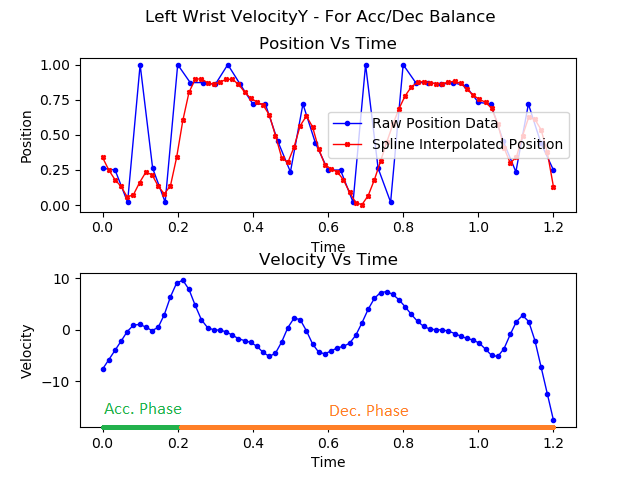
\includegraphics[scale=1]{images/graphs/accDecPhase_Video5_good_LWrist.png}
    \caption{Acceleration and deceleration phases in velocity time graph}
    \label{fig:accDectimes}
\end{figure}

Equation \ref{eq:balance1} shows how the balance between acceleration and deceleration is calculated. In an ideal case, where $t_{acc} == t_{dec}$, the balance is 1, i.e. maximum. 

\begin{gather} 
  B_1 = 1 - \dfrac{|t_{acc} - t_{dec}|}{t_{acc} + t_{dec}}
  \label{eq:balance1}
\end{gather}

However, some researches also suggests that there is no strict rule that the acceleration and deceleration duration should exactly be equal, it is possible that acceleration lasts for more time, hence a new balance score was computed where ideally acceleration time duration is expected to be 20\% more than the deceleration time duration, as described in equation \ref{eq:balance2}. Both these balance scores are then averaged to get a final balance score as shown in equation \ref{eq:balanceFinal}. 

\begin{gather} 
  B_2 = 1 - \dfrac{|t_{acc} - 1.2 \cdot t_{dec}|}{t_{acc} + 1.2 \cdot t_{dec}}
  \label{eq:balance2}
\end{gather}

\begin{gather} 
  B = \dfrac{B_1 + B_2}{2}
  \label{eq:balanceFinal}
\end{gather}

This balance score as described in equation \ref{eq:balanceFinal} can be used as a valid score, but to ease penalty on the user and to standardize every feature to be compared against its corresponding benchmark feature, it is further compared with the balance score of the benchmark to measure how much it deviates from the benchmark's balance score, as shown in equation \ref{eq:scoreBalance}. If the balance of user and benchmark is equal, then the balance similarity score will be 1, i.e. maximum.

\begin{gather} 
  Score_{B} = 1 - |B_u - B_b|
  \label{eq:scoreBalance}
\end{gather}

However, because the keypoints data is not stable, it is possible that the maximum velocity occurs right in the beginning or end of the motion, as shown in figure \ref{fig:accDectimes_maxAtStart}, which is wrong because every user starts motion with an idle position, and ends the motion with deceleration so it the maximum velocity can not occur at the very beginning or end of the motion.

To cater to this issue, we divide the velocity array into $k = 8$ sections, and discard the first and the last section while calculating max velocity. There is no restriction on the value of $k$, however, it should not be very small such that it discards large chunk of values, and should not be very big that it doesn't solve the problem stated. 

\begin{figure}
  \centering
  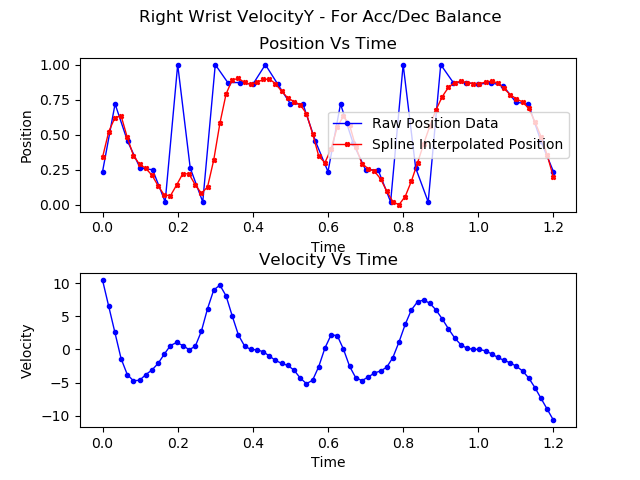
\includegraphics[scale=0.8]{images/graphs/accDecPhase_Video5_good_RWrist.png}
  \caption{Anomalies in velocity affecting balance between acceleration and deceleration}
  \label{fig:accDectimes_maxAtStart}
\end{figure}

The spline interpolation and velocity calculation in figures \ref{fig:accDectimes_maxAtStart} and \ref{fig:accDectimes} are further explained in section \ref{section:filteringSmoothing}

\subsection{Filtering and Smoothing Data}
\label{section:filteringSmoothing}
The common assumption made is that pose estimation is quite accurate however, this is not the case in our project. The raw keypoint data is very jerky and instable due to low net resolution inputted to openpose because of computer hardware constraints as described in section \ref{sub:designConstraints}. The raw data needs to be smoothened to be used further. 


Because of poor pose estimation, the extracted angles are cubic spline interpolated to give smooth results. This has helped improve the angle scores. 

Similarly, for velocity calculation, we can not directly take derivative of keypoint data because the data is very instable and jerky. For velocity calculation, we first ignore the keypoints location whose confidence score is below a minimum threshold, for example, in our case, for any keypoint $i$, we ignored its location from all the frames where its confidence score was below 0.2. The derivative is calculated through Savitzky-Golay filter, but after removing keypoint locations with confidence scores below the minimum threshold, the data becomes unequally spaced, and Savitzky-Golay filter can not be applied directly to this unequally spaced data. To solve this issue, the data is cubic spline interpolated. The cubic spline interpolation smoothes the keypoint data and also makes it equally spaced. 

Savitzky-Golay filter is a digital filter that can be applied to a set of digital data points for the purpose of smoothing the data, that is, to increase the precision of the data without distorting the signal tendency. For velocity calculation, a window size of 7 with order 2 (quadratic) is used to smoothen the data further and extract the derivative through this filter. The window size is selected in a way that the overall trend in the data is not lost and the spikes and jerks in data are removed, keeping nyquist criteria in view. 

\subsection{Dynamic Time Warping}
\label{section:dtw}
To calculate the score based on angles, we can not simply compare them with benchmark angles, as the probability that two users will produce perfectly aligned movements even if they are performing the exact same action, is extremely low. So, even if a user has performed an action exactly like benchmark, it is highly unlikely that there will be frame to frame pose similarity because everyone performs at their own pace, some movements might be slower, some might be faster. Hence, it is impossible to compare frame to frame angles directly. To solve this misalignment issue, dynamic time warping is used to temporally align the frame data of user and benchmark.

For temporally aligning the frames of user and benchmark, a matrix is created which contains the distance (dissimilarity) of each frame of user against each frame of benchmark. For example, given $n$ frames from user's video, and $m$ frames from benchmark video, a dynamic time warping matrix (dtw matrix for short or $\mat D$) is created of order $m \times n$. Each matrix element is computed as the distance between vectors $m_i$ and $n_j$. These vectors are the flattened $18 \times 3$ matrices containing a frame's data. 

\subsubsection{Vector Dissimilarity Computation}
We implemented the following metrics to calculate the distance between each frame vector of benchmark $u$ and user $v$. 

\begin{enumerate}
  \item Cosine distance 
    \begin{align}
       d(u,v) = 1 - \dfrac{u \cdot v}{||u||_2  ||v||_2}
    \end{align}
  \item Correlation
    \begin{align}
      d(u,v) = 1 - \dfrac{(u- \overline{u}) \cdot (v- \overline{v})}{||(u- \overline{u})||_2  ||(v- \overline{v})||_2}
    \end{align}
  \item Euclidean distance
    \begin{align}
      d(u,v) = \sqrt{\sum_{i=1}^{n}(u_i - v_i)^2}
    \end{align}
  \item Absolute difference
    \begin{align}
      d(u,v) =  | u - v |
    \end{align}
\end{enumerate}

We noticed that normalizing the vectors $u$ and $v$ also impacts the distance between these vectors. However, none of these vector distance metrics were working either with or without normalization. This was happening because we were working with the entire frame data for each frame, and because except for a few keypoints, other keypoints either showed very minimal movements or were completely idle. This was making both the vectors $u$ and $v$ very similar and it has hard to compute the key difference between them which was essential for alignment. Hence, we introduced one more metric for computing distance between vectors $yu$ and $v$ which was to select only a subset of keypoints. 

\subsubsection{Optimal Path Calculation}

After creating the matrix, an optimal path from the matrix gives us the temporally aligned frames with maximum similarity. To find the optimal path, we start from matrix item $\mat D_{0,0}$ and move to the neighbour which has the minimum distance of all the immediate neighbours. The minimum distance ensures that we are selecting benchmark and user frame pair which the maximum similarity. Hence, the optimal path gives us the corresponding benchmark frames for each user frame, which had the maximum similarity with it and which also adheres to the temporal arrangement of the frames, i.e. if user frame $v_5$ is mapped to benchmark frame $u_{10}$, then user frame $v_4$ can never be mapped to any benchmark frame $u_i$ where $i > 10$. 

However, starting from $\mat D_{0,0}$ is a very strict requirement because it requires the first frames of both user and benchmark to be similar for the algorithm to work perfectly. For example, it is possible that the user starts the movement one fourth of a second later, in that case, the first frames of user and benchmark are not aligned, and thus the resulting optimal path won't be aligned too because at each step, the algorithm only sees its most immediate neighbours. Hence, the optimal path algorithm starts from any of the first 5 frames of either user or benchmark based on which has the most minimum distance that is maximum similarity. Then, it searches the immediate right, down, and diagonal neighbours and goes to the location where distance value is the minimum. This process repeats until either the rows or columns of the matrix are exhausted. 

From any matrix element $\mat D_{i,j}$, the optimal path algorithm for a single step is described by equation \ref{eq:dtwOptimalPath}.

\begin{align}
  i,j = argmin_{i,j}
  \begin{cases}
    \mat D_{i+1,j}  \\
    \mat D_{i,j+1}  \\
    \mat D_{i+1,j+1} \\
    \label{eq:dtwOptimalPath}
\end{cases}
\end{align}

Figure \ref{fig:dtw_matrix} shows the dynamic time warping matrix constructed, where the columns correspond to user frames and the rows correspond to the benchmark frames, and the optimal path (shown as red) that gives the temporally aligned frames with maximum similarity. 

\begin{figure}
  \centering
  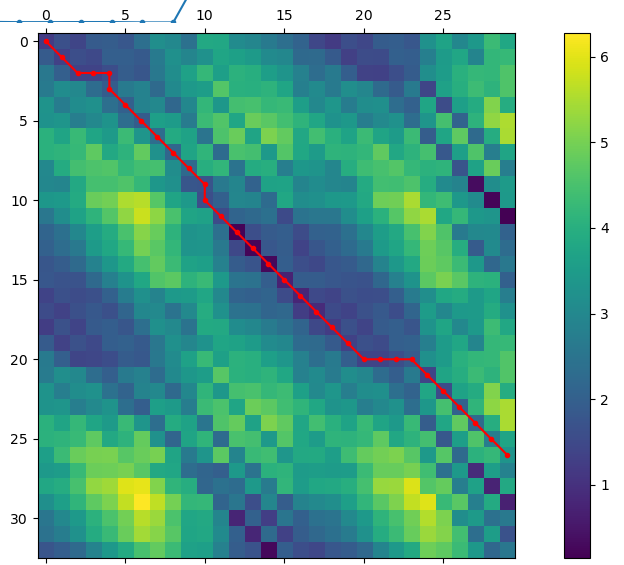
\includegraphics[scale=0.8]{images/graphs/dtw_matrix.png}
  \caption{Dynamic Time Warping Matrix and Optimal Path}
  \label{fig:dtw_matrix}
\end{figure}

\subsubsection{Metrics used in our software}
We found out that the temporal alignment works best on the following parameters.

\begin{enumerate}
  \item Metric = Absolute Difference,
  \item  Normalize = False,
  \item Selected 6 keypoints in frame data only, (right and left) shoulder, elbow and wrists keypoints.
\end{enumerate}

We found that the absolute difference metric outperforms all the other metrics implemented, and because differences are sensitive to magnitudes, not normalizing the vectors works better because they do not alter the magnitudes. Also, because during a punch, the significant movement only happens in these 6 keypoints mentioned above, we need to select only these, otherwise, because other keypoints either show very minimal movements or are completely idle, they average out the entire result and the key differences are lost which are essential for alignment.

\subsubsection{Results of Dynamic Time Warping}

Figure \ref{fig:originalAlignment} shows the original frame to frame alignment without using dynamic time warping for one specific instance in the entire performance. In this original alignment, the blocking action of the benchmark is incorrectly aligned with the punching action of the user. 
However, in figure \ref{fig:optimalAlignment}, which shows the optimal alignment between user and benchmark frame, the blocking action of the benchmark is correctly aligned with the blocking action of the user. 

\begin{figure} 
  \centering
  \subfigure[Benchmark Frame]{% 
    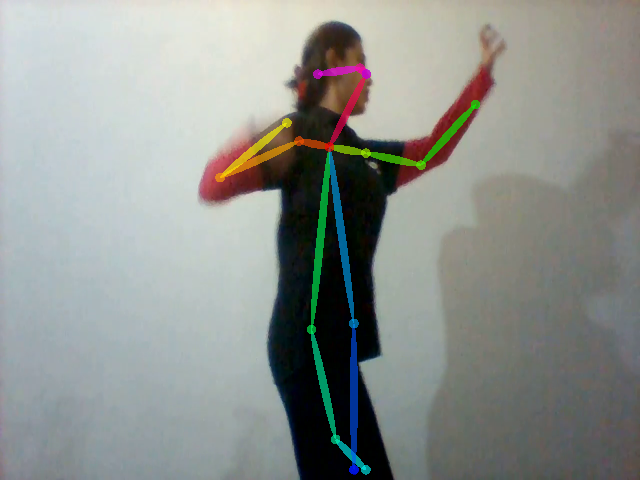
\includegraphics[scale=0.3]{images/dtw_alignment/benchmark_20.png} \label{fig:benchmarkFrame20} 
  } 
 \quad 
  \subfigure[User Frame]{% 
   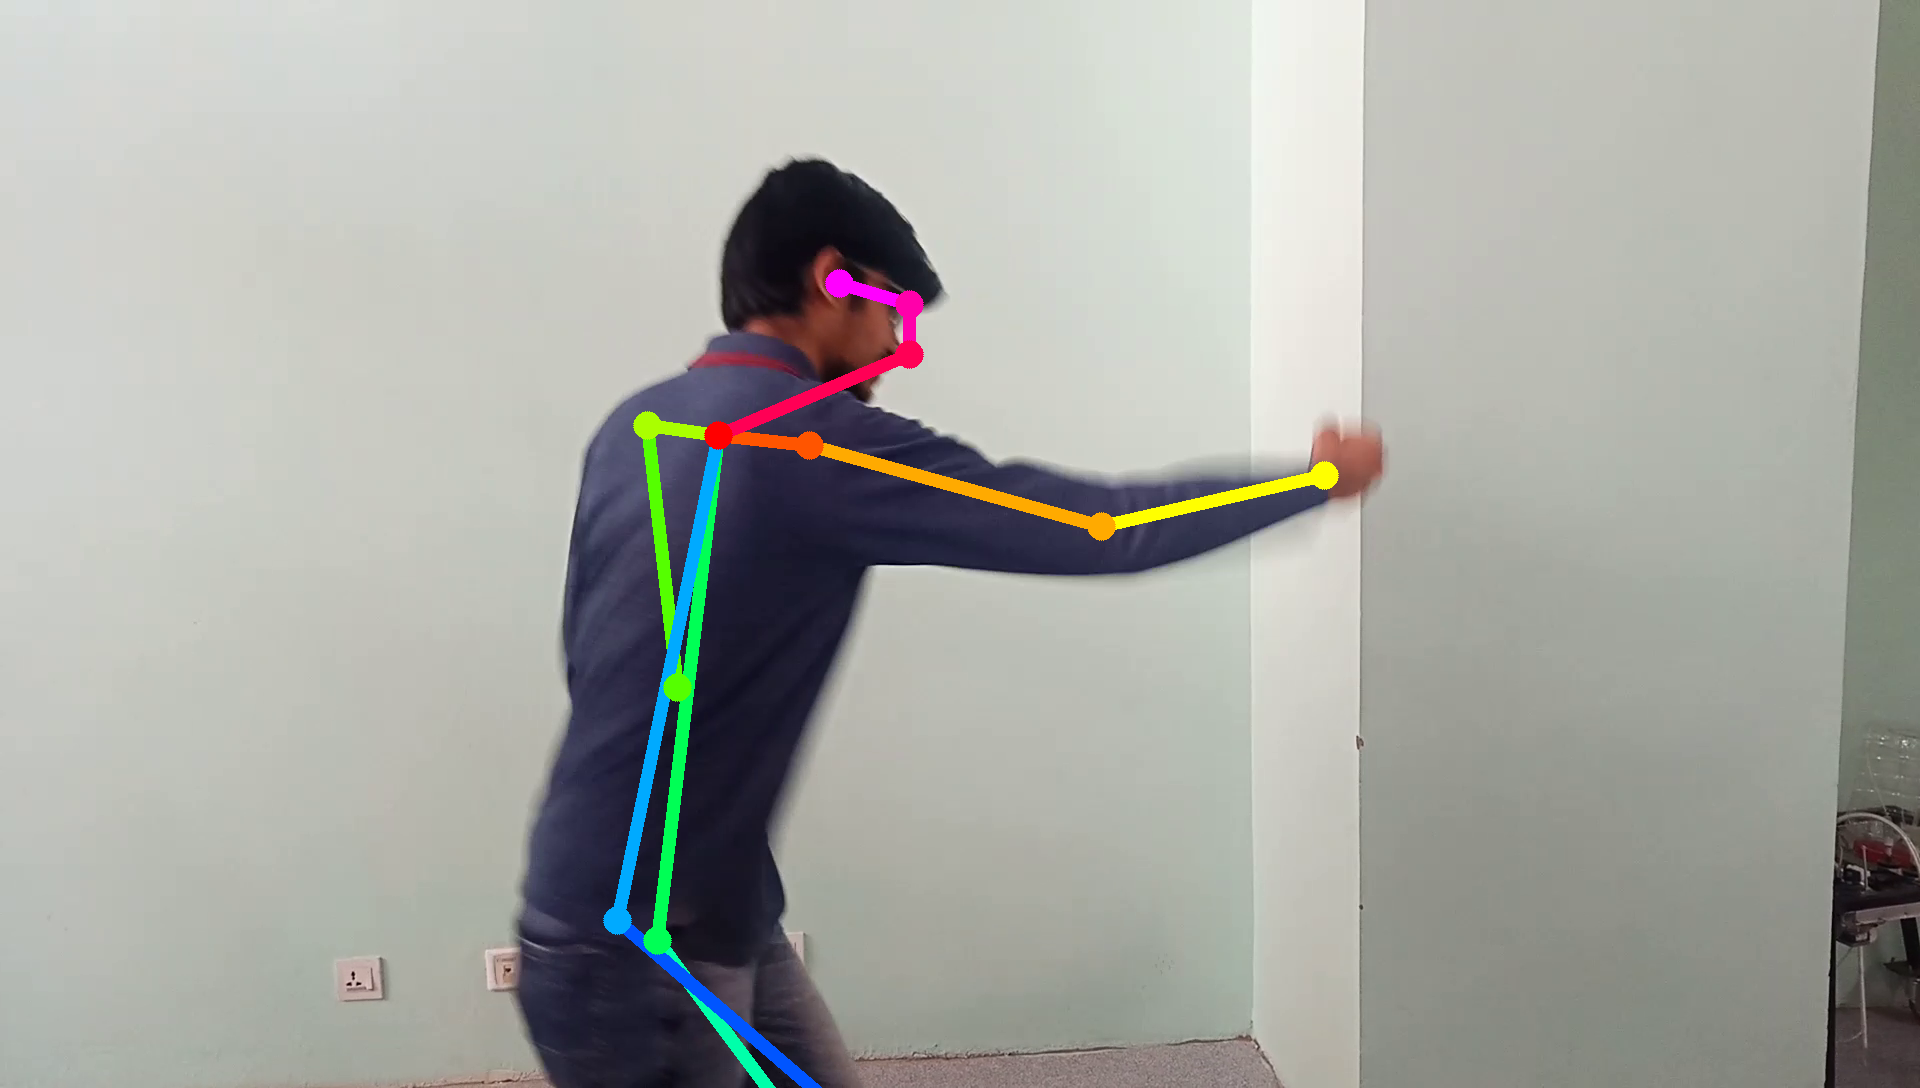
\includegraphics[scale=0.13]{images/dtw_alignment/user_20.png} 
   \label{fig:userFrame20} 
  } 
  \caption{Original Frame to Frame Mapping Without Dynamic Time Warping} 
  \label{fig:originalAlignment}
\end{figure}

\begin{figure} 
  \centering
  \subfigure[Benchmark Frame]{% 
    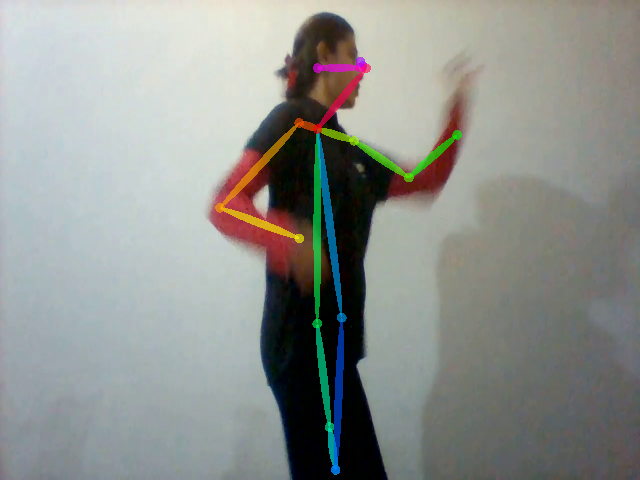
\includegraphics[scale=0.3]{images/dtw_alignment/benchmark_17.png} \label{fig:benchmarkFrame17} 
  } 
 \quad 
  \subfigure[User Frame]{% 
   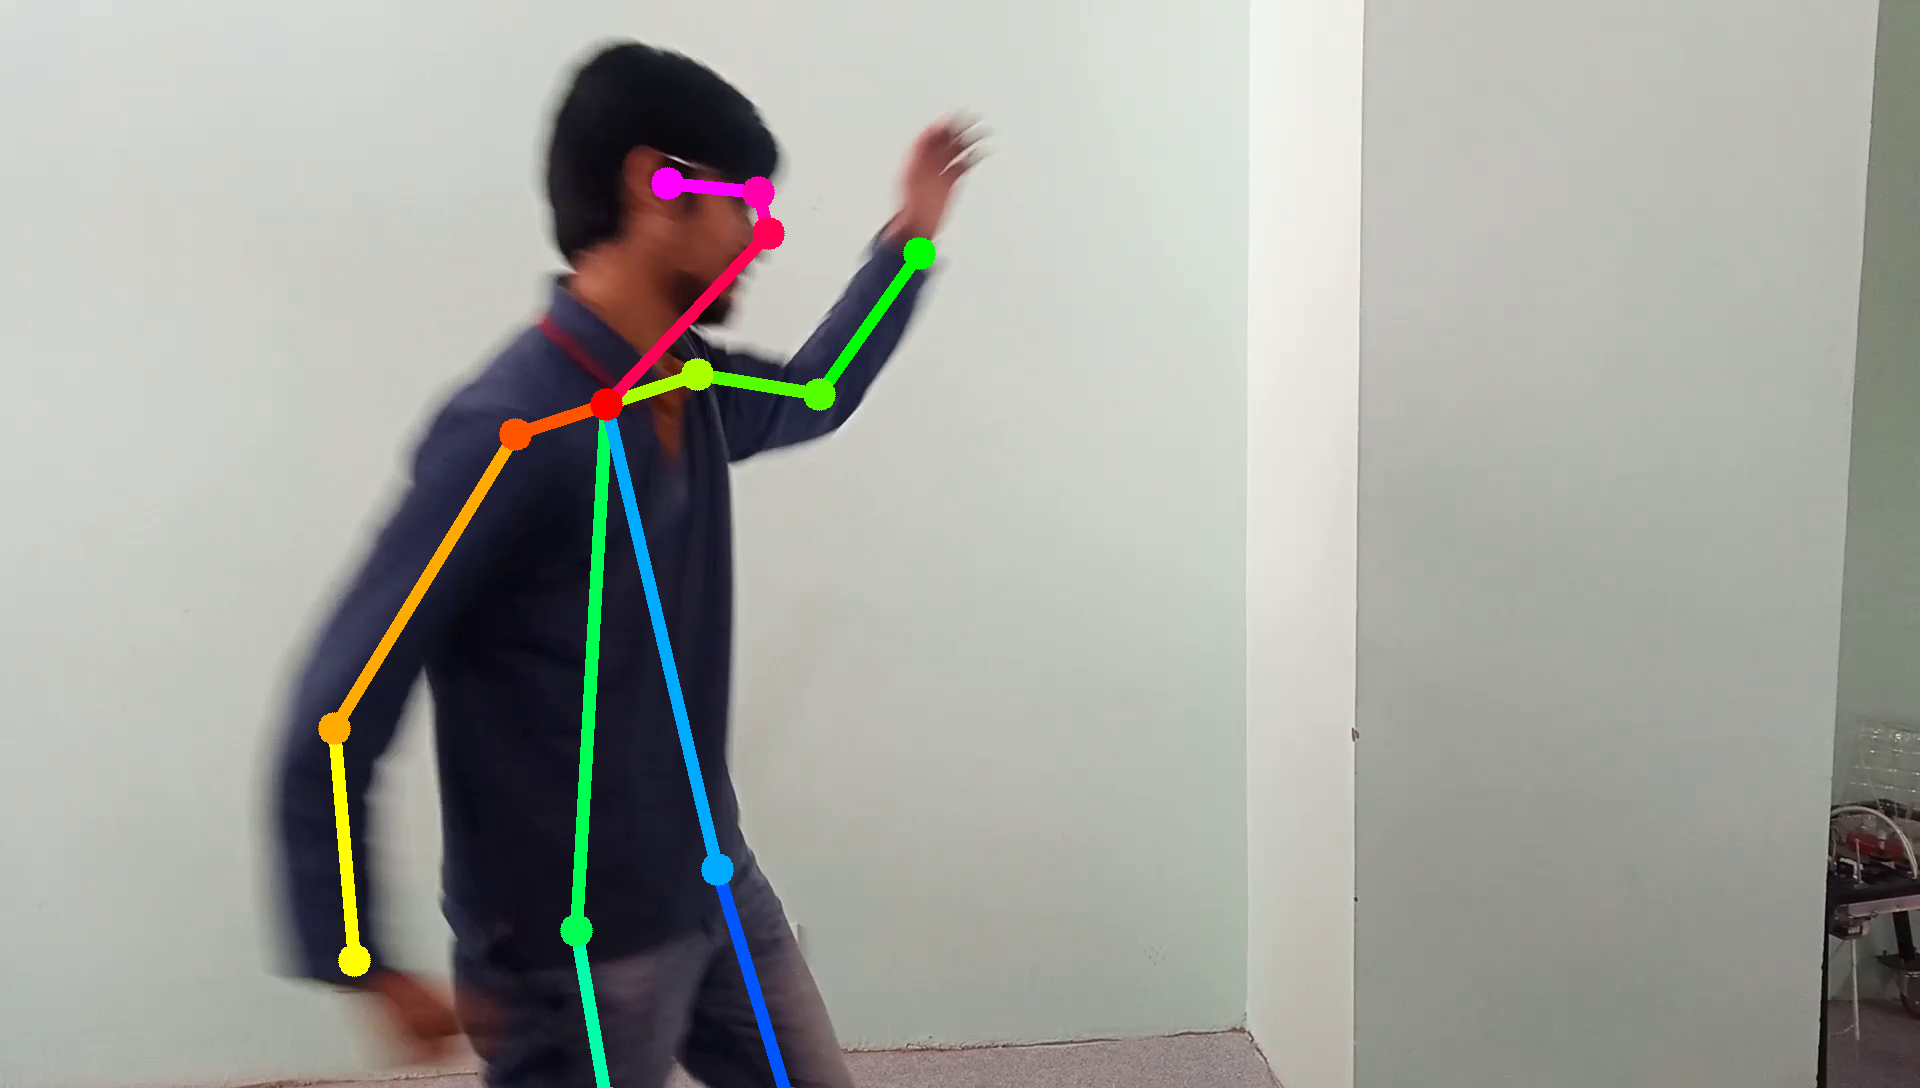
\includegraphics[scale=0.13]{images/dtw_alignment/user_12.png} 
   \label{fig:userFrame12} 
  } 
  \caption{Optimal Frame to Frame Mapping With Dynamic Time Warping} 
  \label{fig:optimalAlignment}
\end{figure}



%In figure (a) we see two lines filtered (red) and unfiltered (blue). The blue sequence is raw data which has anomalies due to incorrect pose estimation. Using confidence scores those values are removed. Now in order to have uniform sampling and further increasing the precision of the data a spline interpolation is performed which further smoothens the data. Without this filtering the final results do not abide by the labels assigned to the datasets. 








 
